\section{Ladder Operator Block-Encoding (LOBE)}
\label{sec:lobe}

In this section of the text, we'll do the following:
\subsection{Defining "Block-Encoding"}
\label{subsec:block-encoding}

\subsection{Prior Works}
\label{subsec:prior-works}

\subsubsection{Linear Combination of Unitaries}

\subsubsection{Sparse Block-Encoding of Pairing Hamiltonians}
stuff from Liu et al
\ws{Might ask you to fill this out @Gus}

\subsection{Circuit Construction}
\label{subsec:circuit}

In Figure \ref{fig:lobe}, we define the LOBE circuit in terms of generic oracles.
Disregarding the (optional) control qubit ($\ket{\textit{ctrl}}$), the LOBE circuit makes use of 5 qubit registers: $\ket{\textit{index}}$, $\ket{\textit{valid}}$, $\ket{\textit{coeff}}$, $\ket{\psi}$, and $\ket{0^{\otimes \alpha}}$.

The register denoted $\ket{\textit{index}}$ is referred to as the index register and is used to index the terms in the Hamiltonian as is done in LCU constructions. 
The integer representations of the computational basis states of the index register corresponds to the indices $l$ in Eq. \ref{eq:lclo}. 
The minimum number of qubits required for this register is given by:
\begin{equation}
    Q_{\textit{index}} = \lceil \log_2{L} \rceil
\end{equation}

The register denoted $\ket{\textit{valid}}$ consists of a single qubit and is referred to as the validation qubit.
It serves the same purpose as in \cite{liu2024efficient} which is to denote whether or not the term at the current index ($T_l$) will annihilate the quantum state.
If the term will annihilate the state, then the validation qubit remains in the $\ket{1}$ state such that the branch of the wavefunction stays outside the desired subspace of the block-encoding.
If the term will not annihilate the state, then the validation qubit gets flipped to the $\ket{0}$ state for the term $T_l$.

The register denoted $\ket{\textit{coeff}}$ is referred to as the coefficient register and is used to apply the coefficients associate with the term $T_l$. 
These coefficients include both the coefficients of the terms in the linear combination ($\alpha_l$) as well as the coefficients associated with the bosonic ladder operators.
One qubit is used to apply the $\alpha_l$ coefficient while a separate qubit will be required for each bosonic operator (defined as a creation, annihilation, or occupation operator acting with a positive integer-valued exponent) in the term.
If we let $K$ denote the maximum number of bosonic operators within a single term, then the number of qubits in the coefficient register is given by:
\begin{equation}
    Q_{\textit{coeff}} = K + 1
\end{equation} 

In addition to the system register - of which the encoding was described in Section \ref{subsec:encoding} - the LOBE cicuit makes use of 5 additional qubit registers.
The top register is a 

\begin{figure}
    \centering
    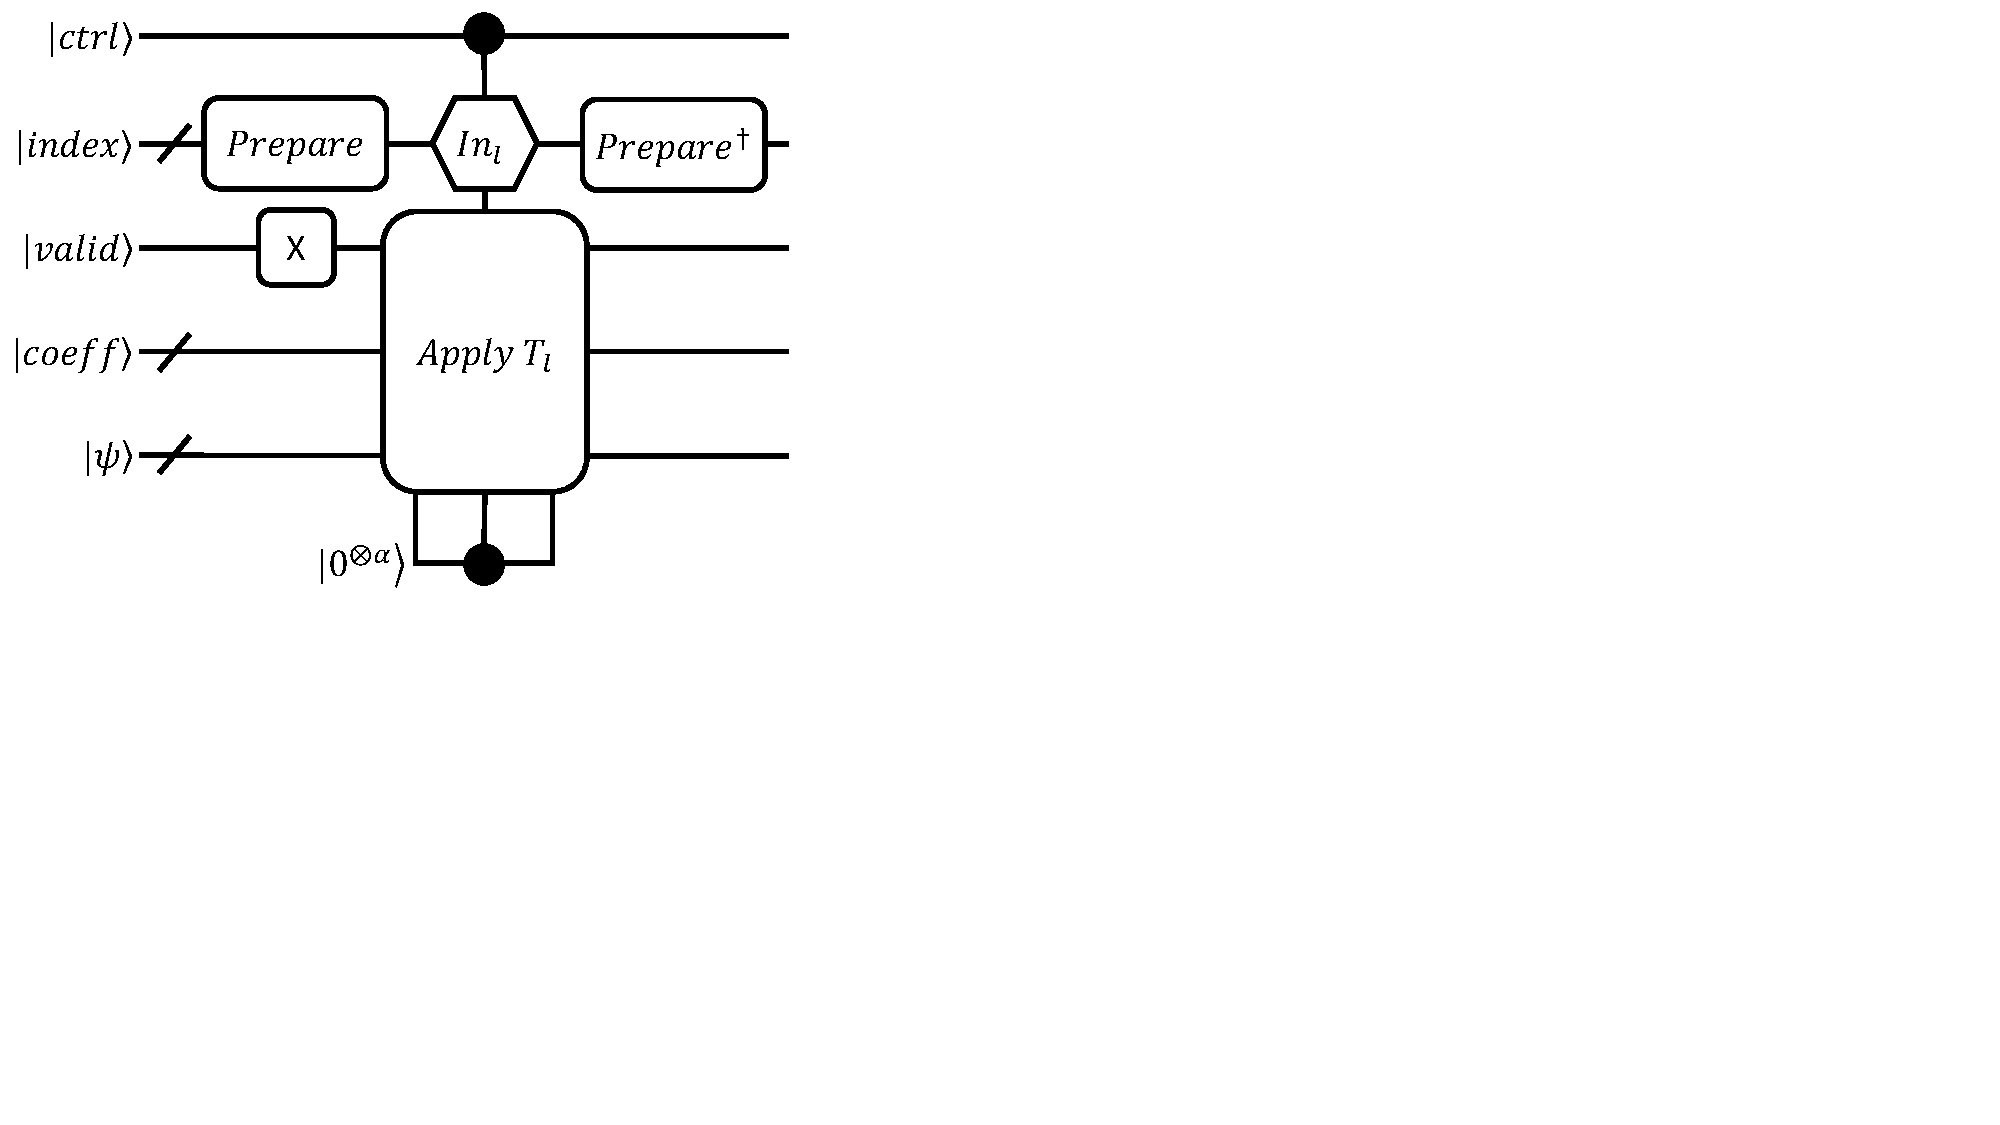
\includegraphics[width=8cm]{figures/lobe-block-encoding.pdf}
    \caption{\textbf{Ladder Operator Block-Encoding.}
    }
    \label{fig:lobe}
\end{figure}

\begin{figure}
    \centering
    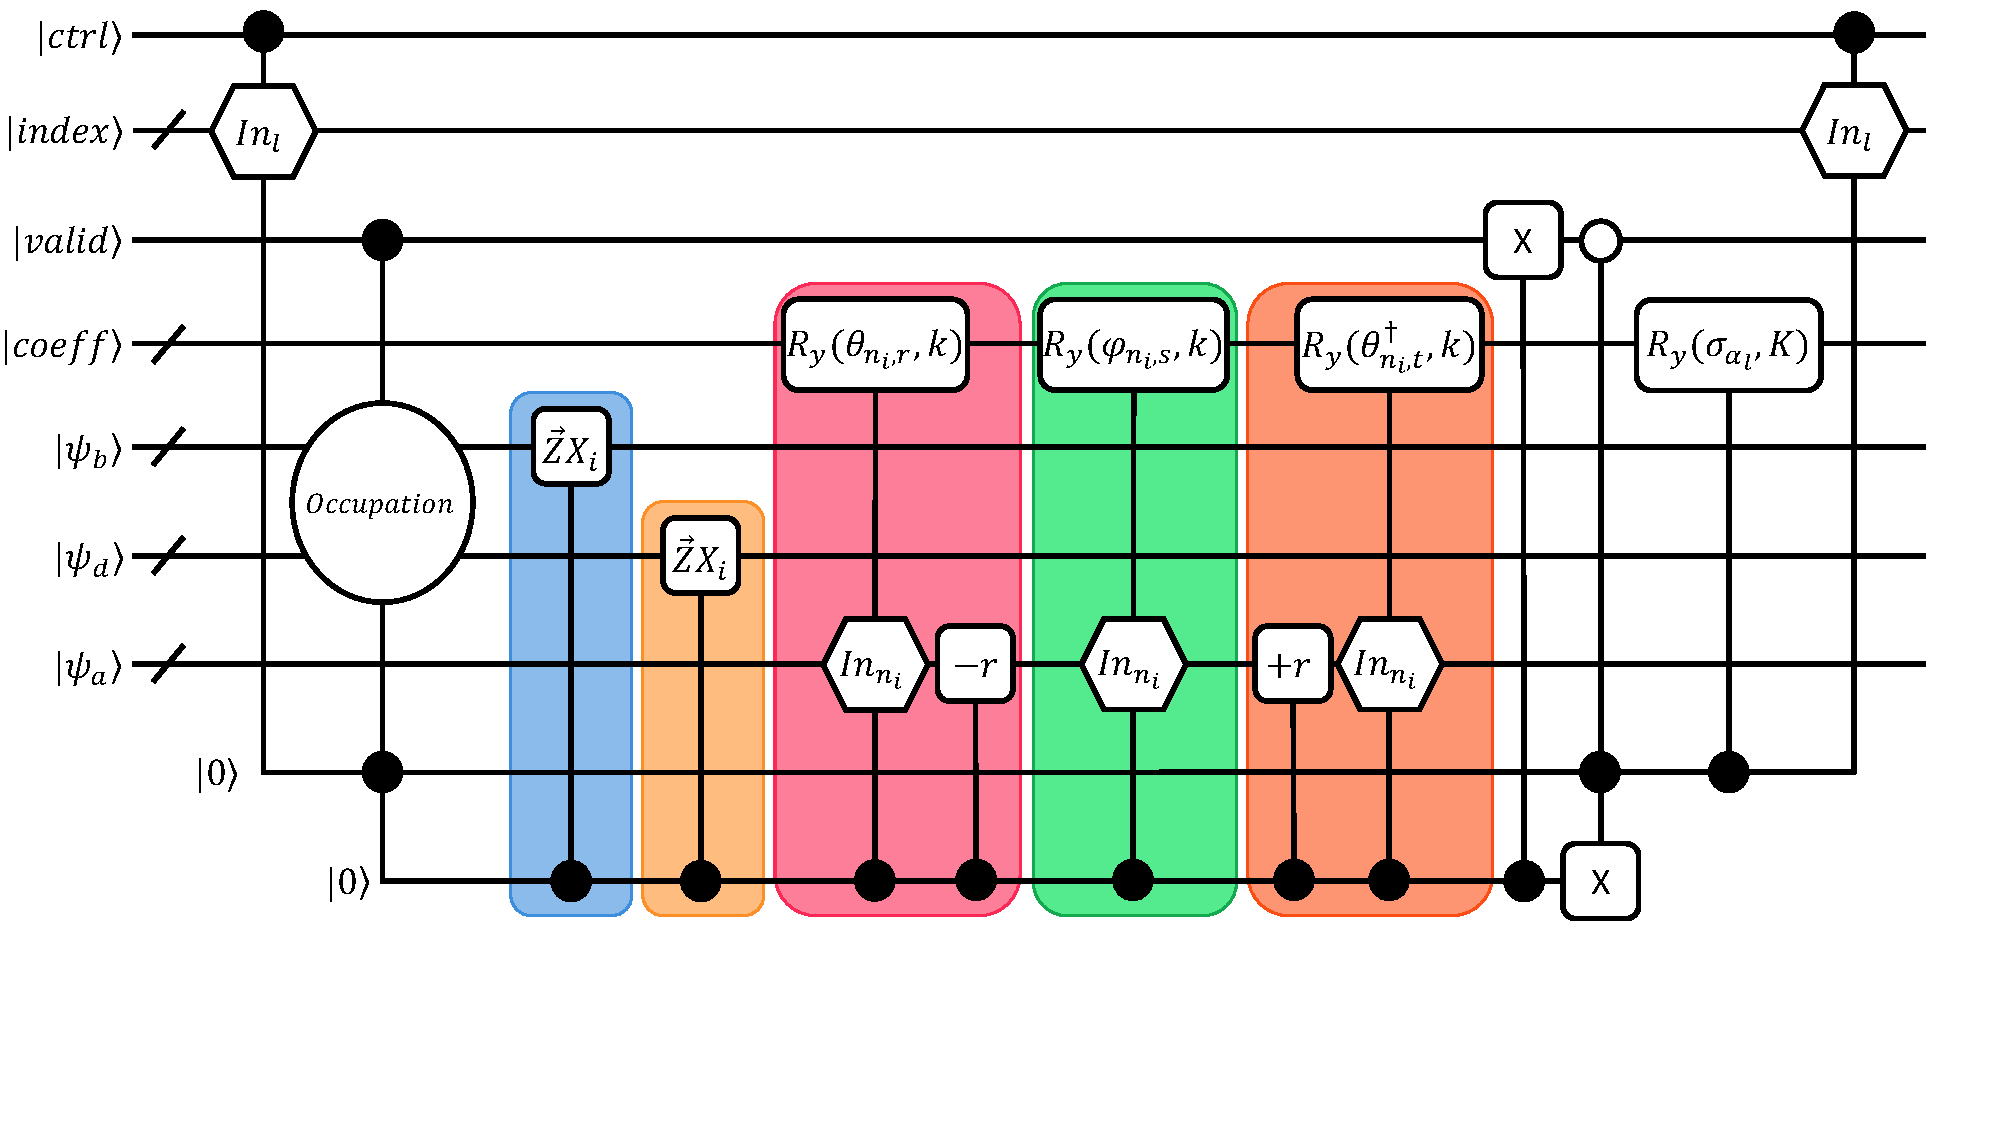
\includegraphics[width=16cm]{figures/applying-term.pdf}
    \caption{\textbf{Ladder Operator Term Oracle.}
    }
    \label{fig:lobe-term}
\end{figure}


\subsection{Hamiltonian Rescaling}
\label{subsec:rescaling}

\subsection{Analytical Cost Analysis}
\label{subsec:analytics}
Detail analytic cost of different variations

\subsection{Example}
\label{subsec:example}
Step-by-step example (intention is to move this to an appendix)
